\documentclass[11pt]{exam}

\usepackage{amsmath}
\usepackage{graphicx}
\usepackage{geometry}
\usepackage{etoolbox}
\BeforeBeginEnvironment{choices}{\par\nopagebreak\minipage{\linewidth}}
\AfterEndEnvironment{choices}{\endminipage}
\geometry{
a4paper,
total={185mm,257mm},
left=10mm,
top=25mm,
bottom=10mm
}

\begin{document}
\setlength{\voffset}{-0.5in}
\setlength{\headsep}{5pt}

\fbox{\fbox{\parbox{8cm}{\centering
\vspace{2mm}
Testat - Versuch D - Zeitabhaengiger Strom - 1
\vspace{2mm}
}}}
\hspace{2mm}
\makebox[0.25\textwidth]{Name:\enspace\hrulefill} \hspace{5mm}
\makebox[0.2\textwidth]{Datum:\enspace\hrulefill}
\vspace{4mm}

\begin{questions}

\question Welche der folgenden Aussagen ist falsch?

\begin{choices}
	\choice Je größer der Widerstand in einem RC-Glied ist, desto kleiner ist die Zeitkonstante. (correct)
	\choice Je größer die Kapazität des Kondensators in einem RC-Glied ist, desto größer ist die Zeitkonstante.
	\choice Die Kapazität eines Kondensators trägt die Einheit Farad.
	\choice Wenn die Spannung an einem Kondensator erhöht wird, bleibt die Kapazität konstant.
	\choice Eine Wechselspannung wird durch Angabe der Signalform, Frequenz, Amplitude und Phase vollständig beschrieben.
\end{choices}

\vspace{3mm}\question Ein zeitlich konstanter Strom \(\mathrm{I=100\,mA}\) fließt in einen Kondensator mit einer Kapazität von \(\mathrm{C=1\,mF}\) und lädt diesen auf. Wie groß ist die Spannung \(\mathrm{U}\) am Kondensator nach der Zeit \(\mathrm{t=10\,s}\)?\(\mathrm{Q=C \cdot U}\) und \(\mathrm{Ampere=Coulomb/Sekunde}\).

\begin{choices}
	\choice \(\mathrm{100\,V}\)
	\choice \(\mathrm{10\,V}\)
	\choice \(\mathrm{1\,kV}\) (correct)
	\choice \(\mathrm{10\,kV}\)
	\choice \(\mathrm{1\,V}\)
\end{choices}

\vspace{3mm}\question Welche Periodendauer hat das auf dem Oszilloskop gezeigte Signal? Der Skalierungsfaktor für die X-Achse beträgt \(\mathrm{0,5\,ms/DIV}\), der Skalierungsfaktor für die Y-Achse beträgt \(\mathrm{1\,V/DIV}\). 

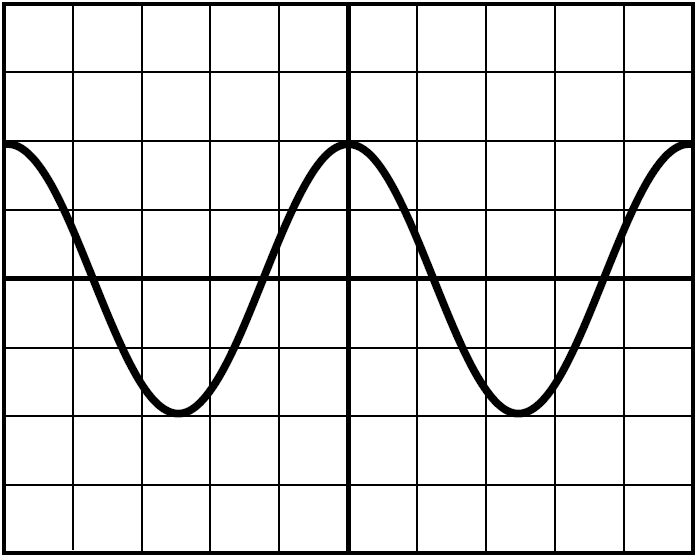
\includegraphics[width=0.5\textwidth]{../../../questions/D/images/Oszi2.png}

\begin{choices}
	\choice \(\mathrm{250\,Hz}\)
	\choice \(\mathrm{2,5\,ms}\) (correct)
	\choice \(\mathrm{5\,ms}\)
	\choice \(\mathrm{0,5\,ms}\)
	\choice \(\mathrm{1\,kHz}\)
\end{choices}

\vspace{3mm}\question Eine Schwingung vollführt in 10 ms genau 100 vollständige Perioden. Wie groß ist die Frequenz?

\begin{choices}
	\choice \(\mathrm{10\,\mu Hz}\)
	\choice \(\mathrm{10\,Hz}\)
	\choice \(\mathrm{10\,kHz}\) (correct)
	\choice \(\mathrm{10\,mHz}\)
	\choice \(\mathrm{10\,MHz}\)
\end{choices}

\vspace{3mm}\question Welcher der folgenden Kurvenverläufe gibt die Entladekurve eines Kondensators über einen konstanten Widerstand qualitativ richtig wieder? 

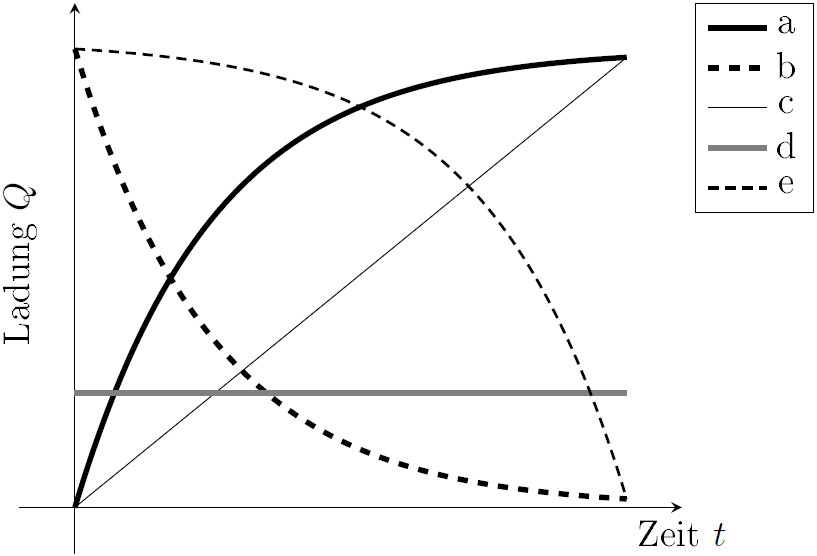
\includegraphics[width=0.5\textwidth]{../../../questions/D/images/Kondensator-Q-t.png}

\begin{choices}
	\choice a
	\choice e
	\choice d
	\choice c
	\choice b (correct)
\end{choices}

\vspace{3mm}\end{questions}

\end{document}
